% !TEX program = pdflatex
% !BIB program = biber
\documentclass[12pt,toc=bib,toc=listof]{scrreprt}
% Shared preamble. Not a main file. The document class is set in bericht/document.tex.
% Four reports include this file, so there is no single `% !TEX root = ...` here.
% LaTeX Workshop only looks for roots under **/bericht/document.tex.

% ------------------------------------------------
% Language & encoding
% ------------------------------------------------
\usepackage[english]{babel}
\usepackage[utf8]{inputenc}
\usepackage[T1]{fontenc}

% ------------------------------------------------
% Layout & typography
% ------------------------------------------------
\usepackage[a4paper,left=30mm,top=25mm,right=25mm,bottom=25mm]{geometry}
\usepackage{lmodern}
\usepackage{microtype}
\usepackage{setspace}
\onehalfspacing

% ------------------------------------------------
% Graphics
% ------------------------------------------------
\usepackage{graphicx}
\usepackage{float}
\usepackage{subcaption}
% Template search paths, plus the shared logo.
% Resolved relative to the bericht/ folder (latexmk working directory).
\graphicspath{{Pictures/}{bilder/}{../../vorlagen/latex/Pictures/}}

% ------------------------------------------------
% Tables
% ------------------------------------------------
\usepackage{booktabs}

% ------------------------------------------------
% Bibliography
% ------------------------------------------------
\usepackage{csquotes}
\usepackage[backend=biber,style=authoryear]{biblatex}
\addbibresource{literatur.bib}

% ------------------------------------------------
% Links
% ------------------------------------------------
\usepackage{xurl}
\usepackage[
  colorlinks=true,
  linkcolor=black,
  citecolor=blue,
  urlcolor=blue
]{hyperref}

% ------------------------------------------------
% Headers and footers (from template 2)
% ------------------------------------------------
\usepackage[headsepline]{scrlayer-scrpage}
\pagestyle{scrheadings}
\clearscrheadfoot
\ihead{\hhnsubject: \reprttopic}
\ohead{\pagemark}
\renewcommand*{\chapterpagestyle}{scrheadings}
\renewcommand*{\chapterheadstartvskip}{}

% Team for all reports. Set once; the title page and PDF metadata read it from here.

\newcommand{\reprtauthoronename}{Teofil Wetzel}
\newcommand{\reprtauthoroneid}{191650}
\newcommand{\reprtauthoronemail}{twetzel@stud.hs-heilbronn.de}
\newcommand{\reprtauthortwoname}{Nick Fronius}
\newcommand{\reprtauthortwoid}{215785}
\newcommand{\reprtauthortwomail}{nfronius@stud.hs-heilbronn.de}

\newcommand{\reprtauthorsblock}{%
  {\large \reprtauthoronename, \reprtauthoroneid}\\[0.4cm]
  {\large \reprtauthoronemail}\\[0.5cm]
  {\large \reprtauthortwoname, \reprtauthortwoid}\\[0.4cm]
  {\large \reprtauthortwomail}%
}

\hypersetup{pdfauthor={Teofil Wetzel, Nick Fronius}}


\graphicspath{{figures/}{Pictures/}{bilder/}{../../vorlagen/latex/Pictures/}}

% ------------------------------------------------
% Document information
% ------------------------------------------------
\newcommand{\hhnfaculty}{Fakultät Wirtschaft und Verkehr}
\newcommand{\hhncourse}{Master Wirtschaftsinformatik (Business Information Systems)}
\newcommand{\hhnprogram}{Winter semester 2026/27}

\newcommand{\hhnsubject}{AI Operations}
\newcommand{\hhnsubjectnum}{}
\newcommand{\hhnlecturer}{Pranav Sharma}

\newcommand{\reprttopic}{News Sentiment Analysis by URL}
\newcommand{\reprttype}{Executive Pitch}
% Authors are listed in vorlagen/latex/autoren.tex.

\begin{document}

% Deckblatt, eingebunden aus bericht/document.tex.
% Kein einzelnes `% !TEX root`: dieselbe Datei gilt für alle vier Berichte.
% ==================================================
% Deckblatt
% ==================================================
\begin{titlepage}
\centering


\includegraphics[width=6cm]{HHN_Logo_D_oS_RGB_300_jpg}\\[1.5cm]

{\Large Hochschule Heilbronn}\\[0.3cm]
{\large \hhnfaculty}\\[1cm]

{\large Studiengang \hhncourse}\\
{\textit{\hhnprogram}\\[2cm]}

{\huge \textbf{\reprttopic}}\\[1.5cm]

{\Large \reprttype}\\[1cm]

\vspace*{1cm}

\reprtauthorsblock\\[1cm]

\begin{flushleft}
\textbf{Modul:}\\
\hhnsubject \\[0.6cm]

\textbf{Dozent:}\\
\hhnlecturer \\[0.6cm]

\textbf{Datum:}\\
\today
\end{flushleft}

\vfill
\end{titlepage}


% scrreprt starts every \chapter on a new page.
% Sections are therefore \section, so the pitch runs continuously.
\renewcommand{\thesection}{\arabic{section}}
\pagenumbering{arabic}

\section{Problem}

Judging the sentiment of news articles by hand is slow, expensive and subjective. Newsrooms, PR \& Communications teams and Analysts have to screen large numbers of articles every day and decide whether the coverage is negative, neutral or positive. Different readers often reach different conclusions, and there is no traceable, repeatable assessment.

Our business goal in the AI Operations module is therefore: given a URL or free text (German and English), automatically return one of three classes --- negative, neutral or positive. The use case is media monitoring and reputation tracking: whoever sees quickly how a topic is coloured in the coverage can react earlier and use resources in a more targeted way.

We framed the project as an MLOps problem on purpose. Training a model once is not enough. We need a reproducible pipeline from the raw article to the API response, a fair model comparison on the same test set, and traceable experiment documentation.

\section{Stakeholders}

Three user groups benefit directly. \textbf{Newsrooms} can triage incoming articles faster and prioritise topics without reading every text by hand. \textbf{PR \& Communications} teams get a signal on their reputation: if negative reports about a brand or an event pile up, this becomes visible early. \textbf{Analysts} use sentiment as an additional indicator in the news flow, for example for market or topic monitoring.

What we deliver is a service interface and evidence that it holds up. The FastAPI endpoints accept either text or a URL (XOR): for a URL, the article body is extracted with Trafilatura, preprocessed and classified. The response contains the predicted class. In parallel, we document the model comparison in MLflow, so that the choice of the production model follows from measurable metrics rather than gut feeling.

\section{Methods}

The pipeline has three steps: scraping or text input, preprocessing (cleaning, tokenisation per model family) and classification into three sentiment classes. The lead metric is macro-F1, so that no class is systematically neglected. Both iterations remain runnable in the repository: the first in \path{src}/ and \path{app}/, the second as the package \path{second_path}.

In the first iteration, five approaches are evaluated on the same financial-sentence test set (PhraseBank English and Kenpache German, split 70\,\% / 15\,\% / 15\,\%, seed~42, $n=1{,}270$):

\begin{itemize}
  \item \textbf{TF-IDF + Logistic Regression} as the classic baseline (macro-F1 0.6562),
  \item \textbf{TF-IDF + LinearSVC} as the best score on this test (macro-F1 0.7202, about 0.02\,ms per text, roughly 4\,MB),
  \item \textbf{\path{tabularisai/multilingual-sentiment-analysis}} as a Hugging Face zero-shot model (macro-F1 0.3636),
  \item \textbf{\path{cardiffnlp/twitter-xlm-roberta-base-sentiment}}, also as a zero-shot comparison (macro-F1 0.4859),
  \item \textbf{DistilBERT fine-tuning}, measured as a CPU subset (2{,}000 sentences, one epoch, context 128; macro-F1 0.6142). The full GPU run in the Colab notebook is described but not measured.
\end{itemize}

The second iteration replaces the word-count vectors with the multilingual encoder \path{paraphrase-multilingual-MiniLM-L12-v2}. First a frozen head (macro-F1 0.6656 on its own test set with $n=1{,}787$), then exactly one fine-tuning of all encoder weights: three epochs, batch 32, context 128, BF16, AdamW, class-weighted cross-entropy. This raises the same test to macro-F1 0.7187. After that come separate ablations within the train split (source-group CV, seed 20261019), without reopening the old test set: R1 weights by language and class, R2 changes chunk aggregation and HTML extraction, R3 stores and computes in BF16, R4 combines the three. R3 is shipped because its CV mean of 0.6729 lies within the pre-defined 0.005 of the best, R4 (0.6740), and the tie rule picks the lower latency (2.381\,ms vs.\ 2.419\,ms) at about 241 instead of 465\,MiB.

Serving and operations: FastAPI with \texttt{/predict} (text or URL, Trafilatura in the first iteration), GitHub Actions for both test paths, MLflow store \path{./mlruns} with the tags \path{iteration=1-first-path} and \path{iteration=2-second-path}. Repository: \url{https://github.com/Rasvan-Teofil/ai-operations-projekt}.

\section{From the first to the second iteration}

In the first iteration, the classic LinearSVC was strong on its financial-sentence test. The transformer attempts were not: zero-shot stays at 0.36 and 0.49 macro-F1, CPU fine-tuning at 0.61, below both TF-IDF models. Performance on more general news was therefore not shown, and the full DistilBERT run was missing.

In the second iteration we changed the approach, not just one number. Instead of TF-IDF a multilingual MiniLM, instead of a short CPU subset a fixed fine-tuning on the full train split, followed by single parameter and operations changes under a selection rule fixed in advance. On the second iteration's own test set, fine-tuning improves on the frozen encoder by 0.0531 macro-F1 (0.6656 to 0.7187) at practically the same inference time. The source CV in Table~\ref{tab:ablation} shows where the change helps and where it does not: the jump lies between the frozen baseline B0 (0.6306) and the reference fine-tune R0 (0.6724, $\Delta +0.0418$). R1 to R4 only move the CV mean in the third decimal place. The clear operational gain of R3 is the halved artefact size.

\begin{table}[H]
\centering
\small
\caption{Source CV in the second iteration, mean over three folds.}
\label{tab:ablation}
\begin{tabular}{lrrrr}
\toprule
Stage & Macro-F1 & DE & EN & MiB \\
\midrule
B0 frozen & 0.6306 & 0.6566 & 0.6059 & 465.1 \\
R0 reference fine-tune & 0.6724 & 0.7053 & 0.6425 & 465.1 \\
R1 language$\times$class & 0.6739 & 0.7076 & 0.6430 & 465.1 \\
R2 article processing & 0.6727 & 0.7053 & 0.6430 & 465.1 \\
R3 BF16, selected & 0.6729 & 0.7062 & 0.6427 & 240.7 \\
R4 combination & 0.6740 & 0.7065 & 0.6441 & 240.7 \\
\bottomrule
\end{tabular}
\end{table}

These CV figures and the two own test sets (0.7202 and 0.7187) are not one shared ranking. The comparison that sees both approaches on the same texts is the external audit run after the selection had already been frozen: 600 English SEntFiN headlines with a unanimous entity label and their German OPUS-MT translation. German is a transfer check there, not a native gold test. Table~\ref{tab:branch} and Figure~\ref{fig:branch} reproduce the values from \path{reports/development/branch_comparison.md}.

\begin{table}[H]
\centering
\small
\caption{Shared external benchmark on 600 headline pairs.}
\label{tab:branch}
\begin{tabular}{lrrrr}
\toprule
Solution & Macro-F1 EN & Macro-F1 DE & ms/text & MiB \\
\midrule
First iteration, reconstructed & 0.4524 & 0.4293 & 0.250 & 4.08 \\
Second iteration v1 & 0.7360 & 0.6458 & 2.335 & 465.14 \\
Second iteration v2 (R3) & 0.7293 & 0.6557 & 2.326 & 240.73 \\
\bottomrule
\end{tabular}
\end{table}

\begin{figure}[H]
\centering
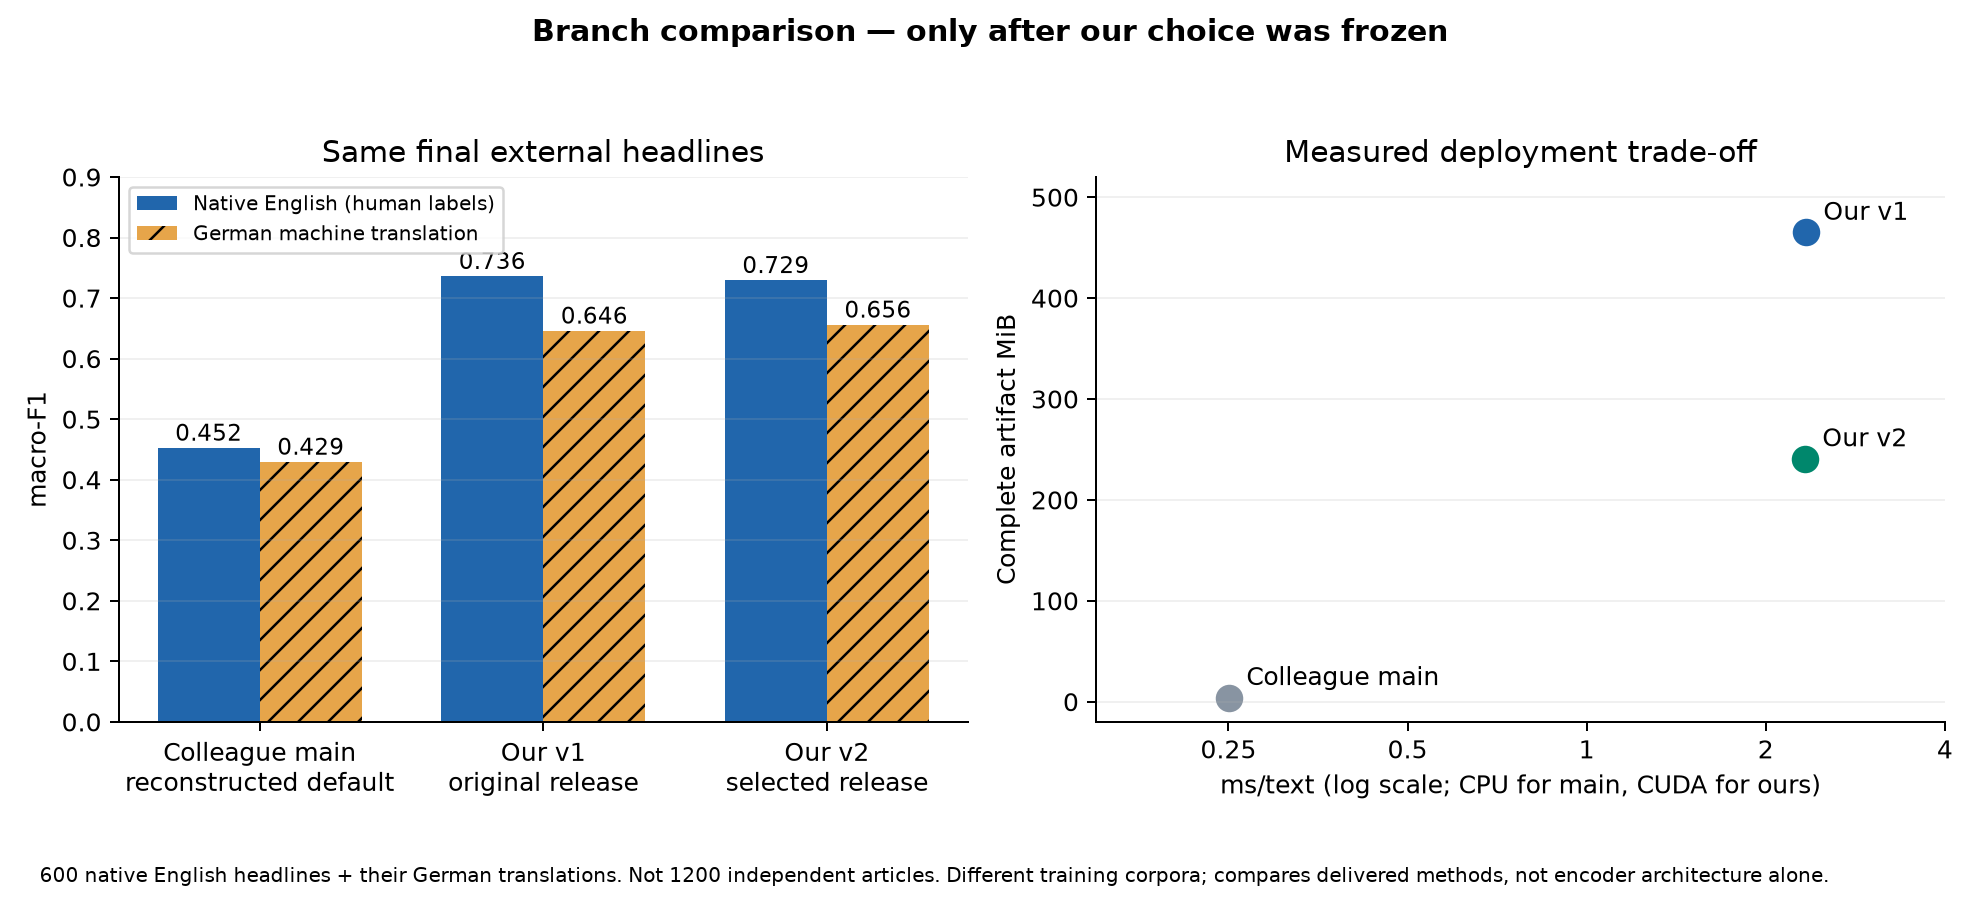
\includegraphics[width=\textwidth]{../../../reports/development/branch_comparison.png}
\caption{External comparison on the 600 headline pairs.}
\label{fig:branch}
\end{figure}

On the native English headlines, v2 is 0.2770 macro-F1 ahead of the reconstructed first default. A paired bootstrap over these 600 already predicted headlines (1{,}000 resamples, seed 20261019) gives a 95\,\% percentile interval for the difference of 0.2257 to 0.3249. v2 is not an across-the-board accuracy gain over v1: English goes from 0.7360 to 0.7293, translated German from 0.6458 to 0.6557. The gain of v2 is the smaller package at similar CV quality. The first default remains much smaller and faster on the CPU. Because the training corpora differ, the audit tests delivered approaches and does not prove an isolated architectural advantage.

\section{Next steps}

The second iteration is measured and documented next to the first in the repository. The full DistilBERT GPU run of the first path is still open; until it is on the test set with $n=1{,}270$, LinearSVC remains the evidenced choice there. R2 and R4 pass the HTML fixtures (six of six instead of two of six), but they are not the API default chosen by the latency rule.

The error costs of a false alarm and of a missed negative report are still not quantified. The training domain remains financial sentences; general coverage, irony and long articles are not covered by evidence. A bias analysis by language or topic remains a lower priority. The local MLflow runs are sufficient for the model choice: live via \texttt{python -m src.train}, and the already recorded GPU metrics without retraining via \texttt{python -m src.import\_recorded}, both in the store \path{./mlruns}. Figure~\ref{fig:mlflow} shows the shared benchmark in the MLflow experiment \path{article-sentiment-comparison}; more screenshots are in \path{docs/mlflow/}.

\begin{figure}[H]
\centering
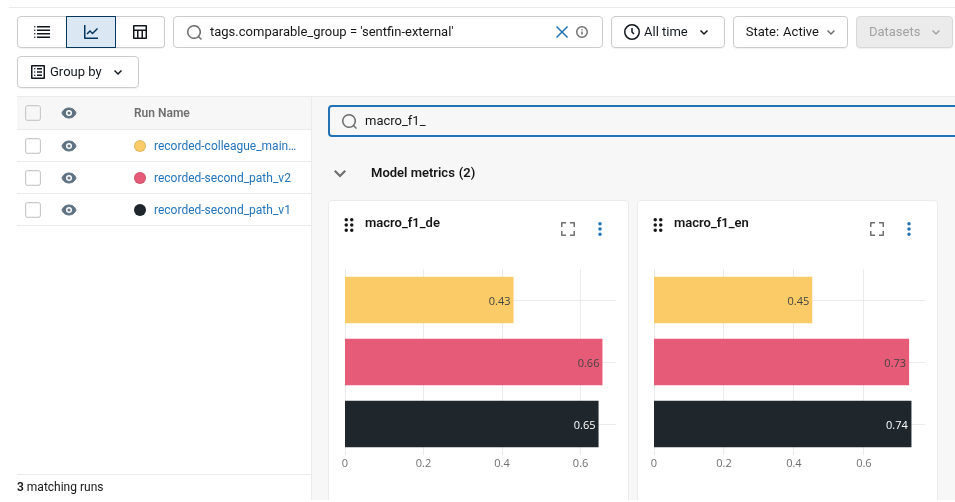
\includegraphics[width=0.55\textwidth]{mlflow_sentfin_chart.png}
\caption{MLflow UI (\texttt{article-sentiment-comparison}): SEntFiN macro-F1, iteration 1 vs.\ 2.}
\label{fig:mlflow}
\end{figure}

In summary: the first iteration delivers a fast, small default and shows that zero-shot and the short CPU fine-tuning do not beat it. The second iteration improves encoder quality on the shared headline benchmark and halves the artefact size with BF16, without redefining the selection rule afterwards.

\end{document}
